\begin{tikzpicture}[auto, scale=.65]
	\tikzset{
		mynode/.style={rectangle,rounded corners,draw=black,fill=TUMBlue!80,very thick, inner sep=1em, minimum size=3em, text centered, minimum width=10cm, text=white, minimum height=1.5cm},
		myarrow/.style={
			->,
			thick,
			shorten <=2pt,
			shorten >=2pt,},
		mylabel/.style={text width=7em, text centered} 
	} 

\usetikzlibrary {arrows.meta}
\definecolor{airforceblue}{rgb}{0.36, 0.54, 0.66}
\definecolor{battleshipgrey}{rgb}{0.52, 0.52, 0.51}
\definecolor{jade}{rgb}{0.0, 0.66, 0.42}
% nonconvex scenario reachability
\draw (-2.5, 3.75) node  [font=\scriptsize, color=airforceblue] [] {Nonconvex };
\draw (-2.5, 3.35) node  [font=\scriptsize, color=airforceblue] [] {Scenario Reachability};
\draw [draw=airforceblue, rounded corners=10, fill=airforceblue, fill opacity=0.1] (-5,0) rectangle (0,4);
% components
\draw (-3.35, 2.25) node  [font=\scriptsize] [] {
$\underset{\theta}{\text{minimize}}$ \hspace*{1mm} $\text{Vol}(\theta)$};
\draw (-4, 1.75) node  [font=\scriptsize] [] {
$\text{subject to}$ };
\draw (-2.4, 1.15) node  [font=\scriptsize] [] {
$\theta \in  \underset{i = 1, ..., N}{\bigcap} \{\theta_i : g(\delta^{(i)}, \theta_i)\leq 0\}$ };

\draw [fill=black,draw=black, fill opacity=0.15] (0,2.15) -- (0.8,2.15) -- (1,2) -- (0.8,1.85) -- (0,1.85)-- cycle;

% reachable set
\draw (4.5, 3.75) node  [font=\scriptsize, color=battleshipgrey] [] {Reachable Set Estimate};
\draw [draw=battleshipgrey, rounded corners=10] (1,0) rectangle (8, 4);
\draw (2.85, 3) node  [font=\scriptsize] [] {Time Instance:};
\node[inner sep=0pt] () at (2.85, 1.5)
    {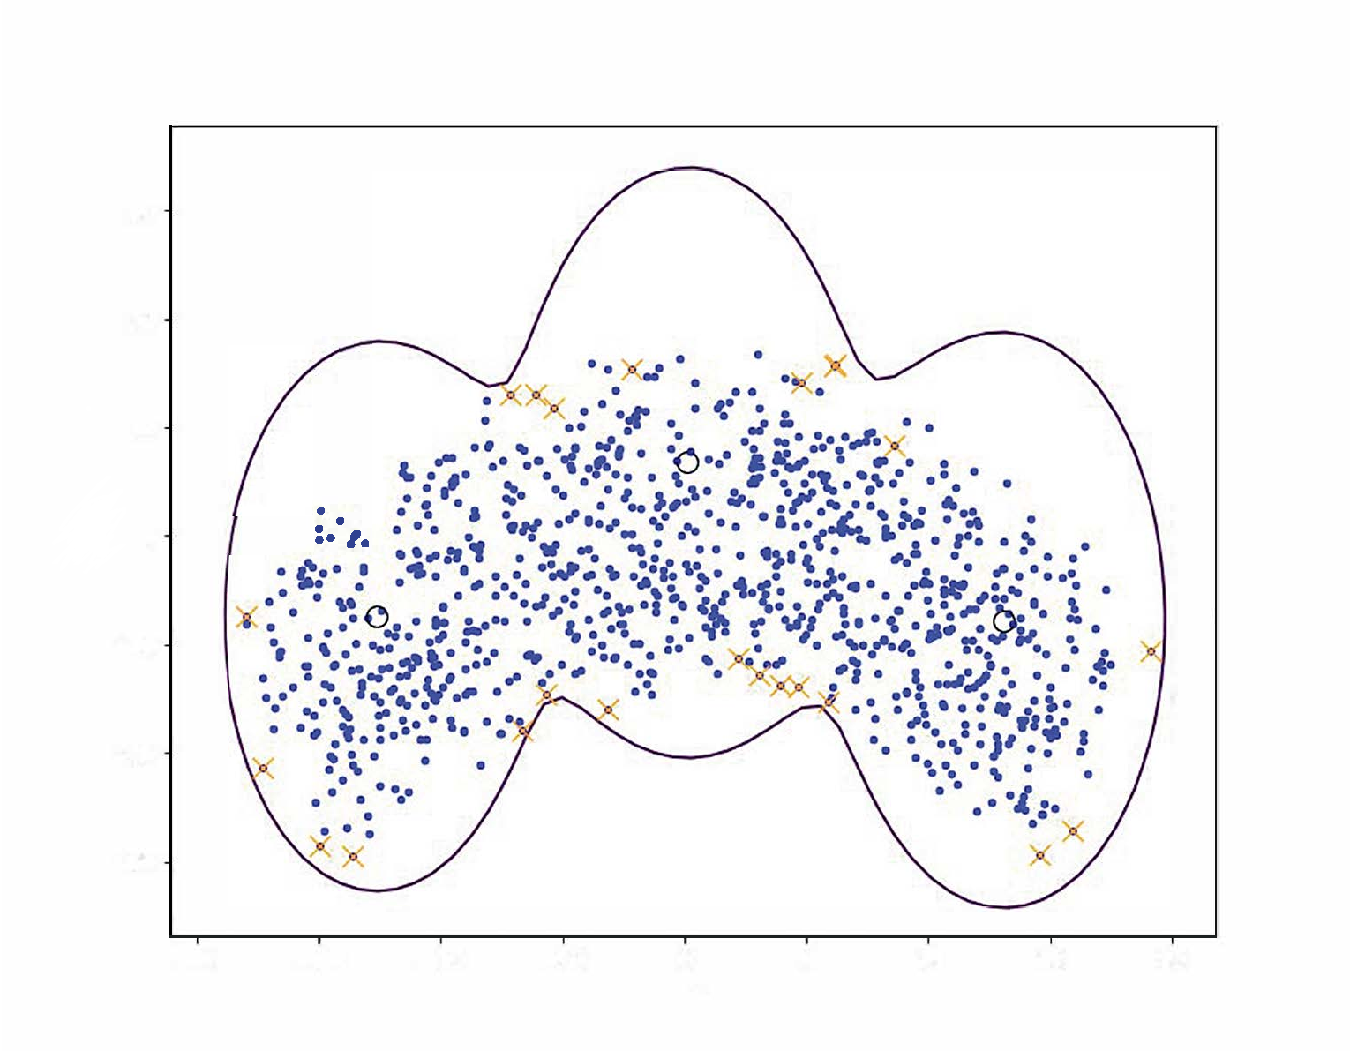
\includegraphics[width=.125\textwidth]{figures/quad_rbf.pdf}};
\draw (6.15, 3) node  [font=\scriptsize] [] {Tube:};
\node[inner sep=0pt] () at (6.15, 1.5)
    {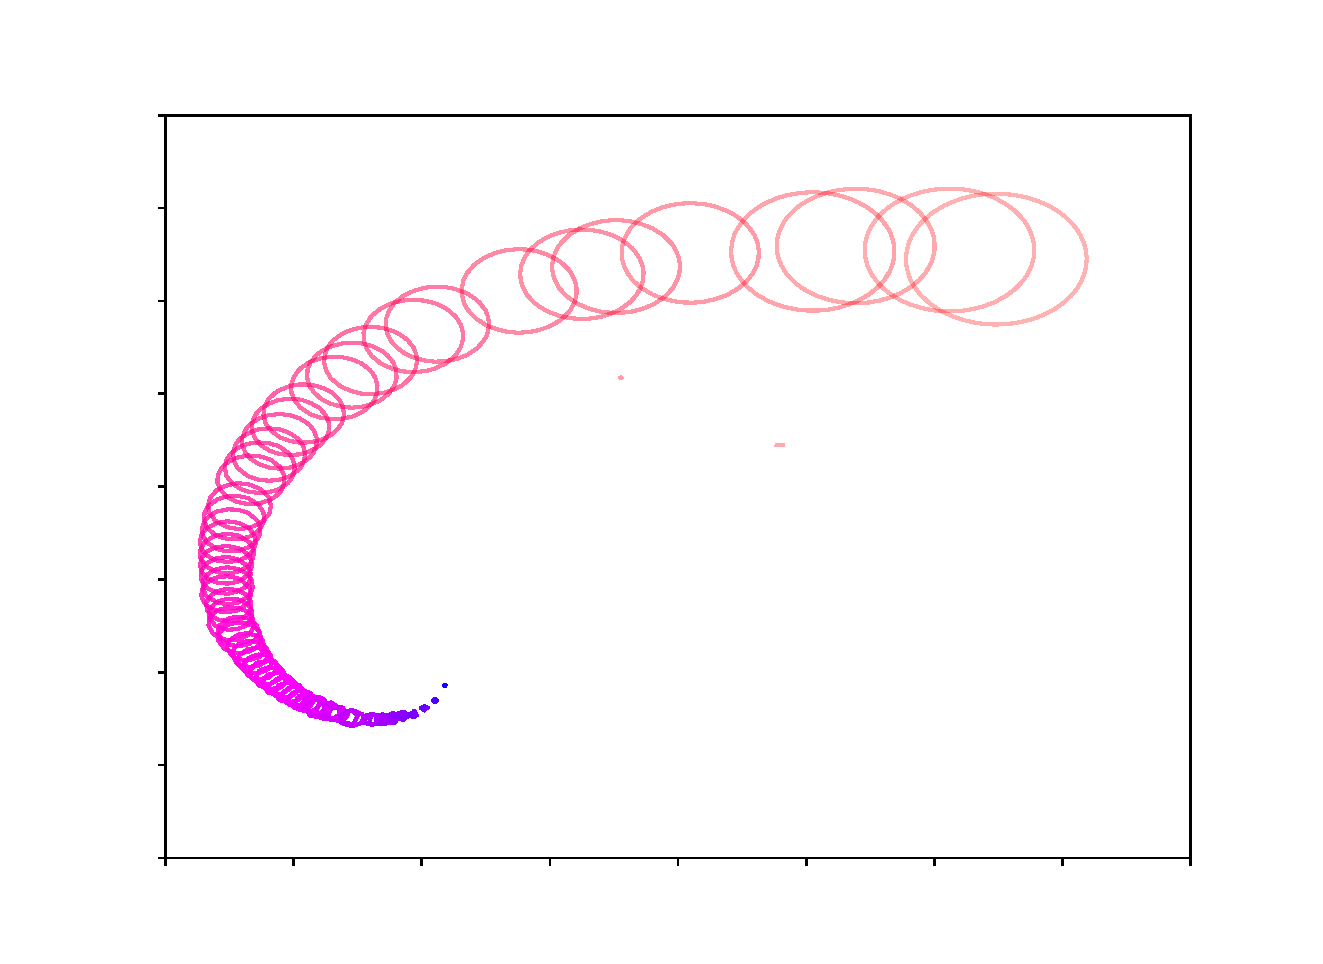
\includegraphics[width=.125\textwidth]{figures/simple_reach_tube.pdf}};

\draw [fill=black,draw=black, fill opacity=0.15] (8,2.15) -- (8.8,2.15) -- (9,2) -- (8.8,1.85) -- (8,1.85)-- cycle;

%Probabilistic Bound
\draw (11.5, 3.75) node  [font=\scriptsize, color=jade] [] {Holdout Method};
\draw [draw=jade, fill=jade, fill opacity=0.1, rounded corners=10] (9,0) rectangle (14, 4);
\draw (11.5, 3) node  [font=\scriptsize] [] {$\mathbf{P} \{ V(\hat{R}(\theta)) > \epsilon\} \leq \beta$};
\draw (11.5, 2.45) node  [font=\scriptsize] [] {$\epsilon :=  \overline{\text{Bin}}(\hat{k}, M, \beta)$};
\node[inner sep=0pt] () at (11.5, 1.15)
    {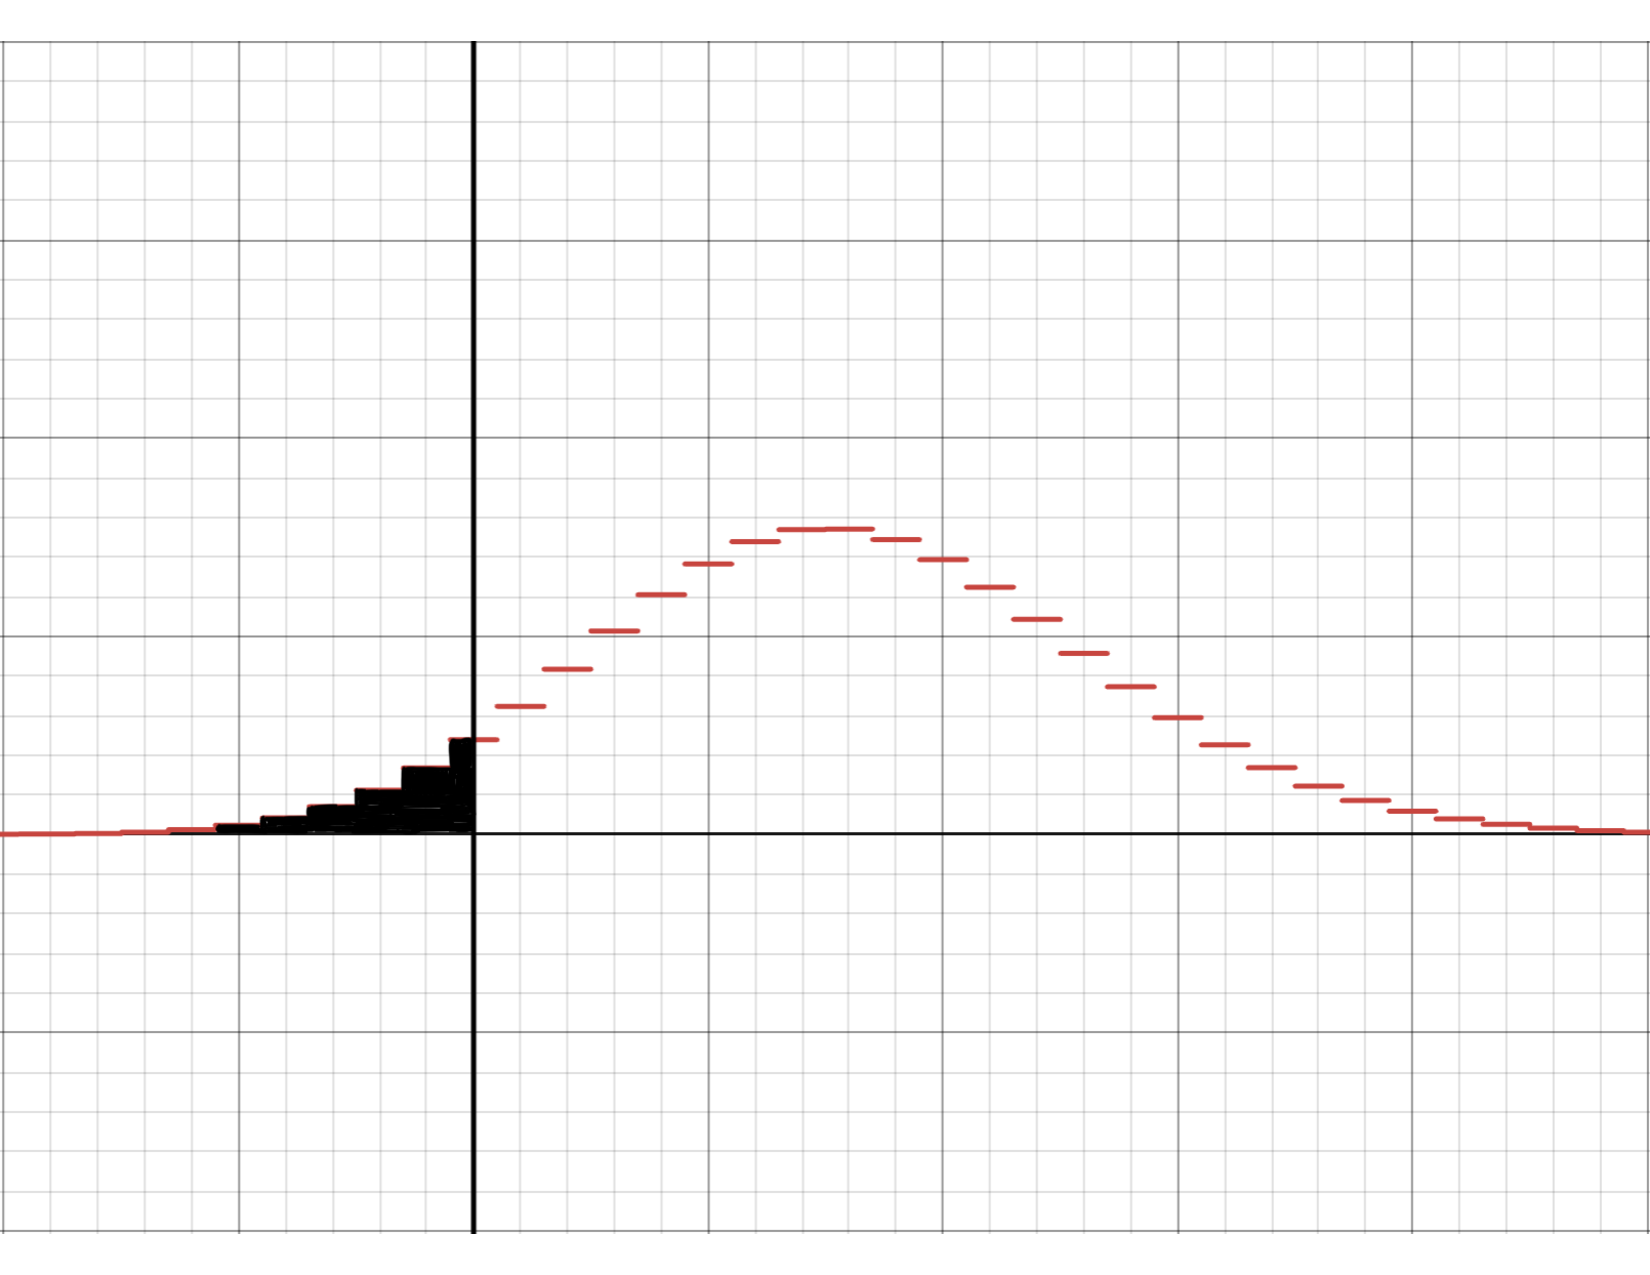
\includegraphics[width=.08\textwidth]{figures/binomial_tail_pic.pdf}};

\end{tikzpicture}